\documentclass[10pt,twocolumn]{article}
\usepackage[a4paper,margin=16mm,columnsep=6mm]{geometry}
\usepackage{amsmath,amssymb}
\usepackage{booktabs}
\usepackage{graphicx}
\usepackage{microtype}
\usepackage{xcolor}
\usepackage{hyperref}
\usepackage{caption}
\usepackage{subcaption}
\usepackage{enumitem}
\usepackage{array}
\usepackage{tabularx}
\usepackage{tikz}
\usetikzlibrary{arrows.meta,positioning,fit}
\hypersetup{colorlinks=true,linkcolor=teal!55!black,citecolor=teal!55!black,urlcolor=teal!55!black}
\graphicspath{{../figures/}}
\captionsetup{font=small,labelfont=bf}
\setlist{nosep,leftmargin=*}
\setlength{\parindent}{1em}
\setlength{\parskip}{0.25em}

\definecolor{mixed}{HTML}{0F766E}
\definecolor{pure}{HTML}{2563EB}
\definecolor{strict}{HTML}{EA580C}
\definecolor{ink}{HTML}{172033}

\title{\vspace{-1.2em}\textbf{Chasing the Nines: Reliability Across States and Seeds}\\[-1mm]\large A Fixed-Grid Pendulum Case Study}
\author{Project 15}
\date{23 July 2026}

\begin{document}
\maketitle
\vspace{-1.6em}

\begin{abstract}
An average return can hide a small but consequential failure tail. We study reliability on a controlled Pendulum benchmark with 2,501 initial states and five independently trained actor seeds. Every reported policy is frozen before the reference is loaded for scoring. Hardcoded angle routers, angle-specific inference rules, reference queries at inference, and mixtures of policy checkpoints are excluded. The selected clean reinforcement-learning-plus-supervision recipe obtains 12,496 near-reference successes from 12,505 seed-state trials, or 99.928\%. The selected pure reinforcement learning recipe obtains 11,832, or 94.618\%. This is an unequal-resource comparison between selected pipelines, not a causal estimate of supervision. The difference is primarily seed-dependent: the mixed method succeeds for all five seeds on 99.680\% of grid cells, compared with 90.164\% for pure reinforcement learning. Paired comparisons support contributions from the follow-up stage, conservative critic search, symmetry projection, and global critic search. Diagnostics suggest that the pure reinforcement learning critic contains useful local action information, but its disagreement is large relative to the correction signal and 19.0\% of tested proposals harm realized return on targeted hard states. The resulting account distinguishes high return, task completion, near-reference reliability, and strict reference wins.
\end{abstract}

\section{Introduction}

This project began with a simple question: what prevents a deep reinforcement learning policy from moving from 90\% success to 99\%, 99.9\%, and the next nine? The practical target changed as the work progressed. The final study compares two routes to reliable control: a mixed route that uses reference actions during training, and a pure reinforcement learning route that learns only from reward. The goal is a policy that works across initial conditions and across random training seeds.

Reliability has two axes here. Within a seed, a policy should cover the full evaluation grid rather than only common reset states. Across seeds, the same state should not alternate between success and failure because of training randomness. This distinction matters because a pooled success rate can conceal a policy family whose difficult states change from seed to seed.

Even in a simple deterministic control task, a five-point average-rate improvement can correspond to hundreds of seed-state failures and large training-seed variability. The selected mixed pipeline reaches 99.928\% near-reference success, compared with 94.618\% for the selected pure-RL pipeline.

This pipeline synthesis and reliability audit makes four contributions. First, it audits all standardized evaluations in two experiment repositories and applies one legality rule and one evaluation protocol. Second, it identifies the best completed clean automatic-priority mixed and pure-RL pipelines at 100,000 learning transitions or fewer under the selected-route ledger. This ledger does not equalize full-study cost, discovery interactions, reference queries, or complete-pipeline replication. Third, the study decomposes both winners with paired ablations. Fourth, it uses hard-state critic diagnostics and cross-seed maps to investigate the performance gap without treating exploratory measurements as established causes.

\section{Related work}

\paragraph{Soft Actor-Critic.}
Soft Actor-Critic, or SAC, learns a stochastic actor and twin value critics while maximizing reward and entropy \cite{haarnoja2018sac}. Twin critics reduce optimistic value errors. In this project, categorical SimbaV2 critics represent a distribution over bounded return atoms rather than only a scalar mean.

\paragraph{DAgger and learner-state coverage.}
Dataset Aggregation, or DAgger, repeatedly lets the learner control the system, labels the visited states with a reference policy, and adds those examples to the training set \cite{ross2011dagger}. This procedure directly addresses compounding error under distribution shift. Our mixed pipeline adds an automatic start-selection stage that ranks uniformly sampled candidates by measured regret. No angle interval is written into the training code.

\paragraph{Normalized residual networks.}
SimbaV2 uses hyperspherical normalization and residual structure to stabilize scalable deep reinforcement learning \cite{lee2025simba}. Both winning actors use SimbaV2 backbones, although the matched DAgger backbone ablation shows that the architecture name alone does not explain the result.

\paragraph{Multi-step SAC critics.}
SACn trains SAC critics with multi-step returns \cite{lyskawa2025sacn}. FastSACN reduces the number of active horizons. The historical FastSACN8 critic used by the mixed method activates one-step and eight-step endpoints with $\lambda=0.5$. The normalized nominal weight of the eight-step endpoint is only $0.5^7/(1+0.5^7)=0.7752\%$. It is therefore mostly a one-step critic with a small long-horizon auxiliary. This detail prevents an unsupported conclusion that eight-step credit assignment caused the mixed result.

\paragraph{Reliable evaluation and hybrid improvement.}
Deep reinforcement learning comparisons are sensitive to random seeds, implementation choices, and aggregate statistics \cite{henderson2018matters,agarwal2021precipice}. We therefore report exact paired grid counts and cross-seed cell consistency instead of only a mean and standard error. Demonstration-augmented policy gradients provide a related route for combining imitation and reward optimization \cite{rajeswaran2018dapg}. Critic-guided action optimization has also been used in large-scale continuous-control systems such as QT-Opt \cite{kalashnikov2018qtopt}. Our deployment search differs by using a fixed candidate set and an explicit twin-critic agreement gate.

The broader design space includes tail-sensitive objectives, automatic hard-start curricula, equivariant actors and critics, uncertainty-gated action selection, and distillation of searched actions back into an actor. Our experiments isolate one representative of the curriculum, symmetry, and uncertainty-gating ideas. They do not compare risk-sensitive training objectives or complete a search-distillation study.

\section{Problem and protocol}

\subsection{Environment and evaluation grid}

The observation is
\[
s=(\cos\theta,\sin\theta,\dot{\theta}),
\]
and the bounded torque is $a\in[-2,2]$. Each deterministic evaluation lasts 200 steps. The grid contains 61 angles in $[-\pi,\pi]$ and 41 angular velocities in $[-1,1]$, giving 2,501 states. Five independently trained actor seeds produce 12,505 seed-state trials for each method.

The environment is Gymnasium \texttt{Pendulum-v1} under a 200-step time limit with no early terminal state. Its raw step reward is
\[
r_t=-\left(\theta_t^2+0.1\dot{\theta}_t^2+0.001a_t^2\right),
\]
where $\theta_t$ is wrapped to $[-\pi,\pi]$. The reported return is the undiscounted 200-step reward sum. Actor seed identifiers are 0 through 4. The study uses the implementation's registered SimbaV2 initialization and optimizer defaults; exact configuration files accompany the artifacts.

Two stored reference solvers provide returns $R_{\mathrm{DP}}(s)$ and $R_{\mathrm{ctrl}}(s)$. The scoring reference is
\[
R^\star(s)=\max\{R_{\mathrm{DP}}(s),R_{\mathrm{ctrl}}(s)\}.
\]
The references are a stored dynamic-programming solution and a stored controller solution evaluated on the same initial condition. They are strong comparators, not a certificate of global optimality. Strict wins demonstrate that this reference is fallible.
Near-reference success and a strict reference win are
\begin{align}
\mathcal{N}(s)&=\mathbb{1}[R_\pi(s)\geq R^\star(s)-5],\\
\mathcal{B}(s)&=\mathbb{1}[R_\pi(s)>R^\star(s)].
\end{align}
Task success requires at least 80\% of steps near upright and no failure streak longer than 50 steps. A step is near upright when $\cos\theta_t\geq0.95$ and $|\dot{\theta}_t|\leq1$.

The reference is absent from both winning deployments. It is loaded only after each actor and inference rule are frozen. The grid trials are correlated because neighboring states are similar. Counts describe this fixed grid exactly; they are not treated as 12,505 independent population samples.

\subsection{Legality and budget}

A clean method cannot use a hardcoded angle range for training or inference, an angle router, reference values at inference, or a mixture of trained policy checkpoints. Uniform full-circle sampling is legal. Automatic selection based on measured performance is legal. Q-search is legal when the same reference-free rule is applied at every state.

Under the conventional selected-lineage ledger, the mixed route assigns 30,000 learner-controlled DAgger transitions, 20,000 automatic-priority DAgger transitions, and one shared 50,000-transition reward-only critic to each evaluated actor route. The priority stage also spends 800,000 simulator steps per actor seed to score candidate starts. This convention gives 100,000 learning transitions and 900,000 total simulator interactions per selected route, but it repeats the shared critic in each route. Across the actual five-actor study, the mixed method uses 300,000 learning transitions: $5\times50,000$ actor transitions plus one 50,000-transition critic. Its automatic-priority discovery cost is 4,000,000 additional interactions.

\begin{table*}[t]
\centering
\caption{Resource ledger for the headline comparison. ``Route'' assigns the shared mixed critic to one actor lineage. ``Full'' counts the critic once across the five evaluated actors. Reference labels include static and learner-state action queries.}
\label{tab:resources}
\scriptsize
\begin{tabularx}{\textwidth}{>{\raggedright\arraybackslash}p{27mm}rrrrrX}
\toprule
Pipeline & Learn/route & Learn/full & Discover/full & Ref./full & Updates/full & Replication unit\\
\midrule
Automatic-priority mixed & 100k & 300k & 4.00m & 3.45m & 319,810 & Five actors, one shared critic\\
Uniform-start mixed control & 100k & 300k & 0 & 3.45m & 319,810 & Five actors, one shared critic\\
Pure-RL winner & 100k & 500k & 0 & 0 & 495,000 & Five complete actor-critic runs\\
\bottomrule
\end{tabularx}
\end{table*}

Each mixed actor uses 44,362 minibatch updates. The shared critic uses 98,000 updates, giving 319,810 full-study updates. Each pure-RL seed uses 99,000 updates. The automatic-priority mixed result and pure-RL result are matched only under the selected-route learning ledger. Full-study interaction, discovery, supervision, and update costs are unmatched. The uniform control reaches 12,486 of 12,505 near-reference trials, or 99.848\%, without discovery interactions. The uncertainty reported later is across actor seeds and does not represent five independently repeated mixed pipelines.

Two historical results reached 12,500 of 12,505 near-reference successes, or 99.960\%. One used a 300,000-step selected lineage and manually chosen training neighborhoods. The other used a 280,000-step lineage plus 8,000,000 discovery rollout steps per actor seed. The 99.960\% result was excluded because of budget, and the targeted recipe also violated the current prohibition on hand-selected training regions.

\section{Methods}

\subsection{Mixed training in simple language}

The winning mixed method has five parts. A SimbaV2 actor first learns reference actions across full-circle states. DAgger then labels states reached by the actor itself. A follow-up stage samples candidate starts uniformly and trains on the largest measured mistakes. The supervised target stays equal to the reference action. At deployment, a reward-trained critic checks the actor action and four nearby alternatives. A replacement is accepted only when both critics agree.

\begin{figure*}[t]
\centering
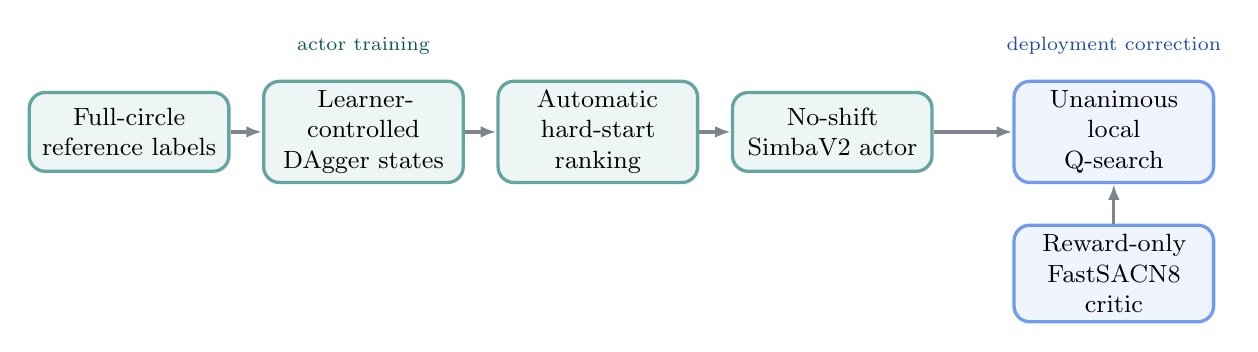
\begin{tikzpicture}[
  node distance=5mm and 4mm,
  every node/.style={font=\small,align=center},
  box/.style={rounded corners=2mm,draw=ink!25,very thick,fill=white,minimum height=10mm,text width=23mm},
  train/.style={box,fill=mixed!7,draw=mixed!65},
  deploy/.style={box,fill=pure!7,draw=pure!65},
  arrow/.style={-{Latex[length=2mm]},very thick,draw=ink!55}
]
\node[train] (static) {Full-circle\\reference labels};
\node[train,right=of static] (dagger) {Learner-controlled\\DAgger states};
\node[train,right=of dagger] (priority) {Automatic\\hard-start ranking};
\node[train,right=of priority] (actor) {No-shift\\SimbaV2 actor};
\node[deploy,right=10mm of actor] (local) {Unanimous local\\Q-search};
\node[deploy,below=5mm of local] (critic) {Reward-only\\FastSACN8 critic};
\draw[arrow] (static) -- (dagger);
\draw[arrow] (dagger) -- (priority);
\draw[arrow] (priority) -- (actor);
\draw[arrow] (actor) -- (local);
\draw[arrow] (critic) -- (local);
\node[font=\scriptsize,text=mixed!75!black,above=2mm of dagger] {actor training};
\node[font=\scriptsize,text=pure!75!black,above=2mm of local] {deployment correction};
\end{tikzpicture}
\caption{The mixed pipeline trains one actor from supervised labels, then uses a separately reward-trained critic as a conservative local action corrector. The critic is not a router and no second actor is mixed into the policy.}
\label{fig:pipeline}
\end{figure*}

\subsection{Mixed training details}

The width-64, two-block SimbaV2 actor is initialized from 400,000 reference-labelled states. Sixty percent use full-circle angles and velocities in $[-1,1]$; forty percent use full-circle angles and velocities in $[-8,8]$. Training uses 80 epochs, batch size 1,024, and learning rate $3\times10^{-4}$. Three learner-only DAgger rounds add 10,000 transitions each, followed by ten training epochs after each round. The learner always executes, so the DAgger mixture coefficient is $\beta=0$. The initializer uses 43,600 optimizer steps. Its terminal epoch 110 checkpoint minimizes stored validation action MAE.

The follow-up creates 240,000 new reset-support labels. It samples 4,000 candidate starts uniformly and scores
\[
\rho(s_0)=R^\star(s_0)-R_\pi(s_0).
\]
It selects the 90 largest-regret starts and 10 uniformly chosen remaining starts, then collects one 200-step learner-only trajectory from each. The resulting 260,000-example dataset is trained for three epochs at learning rate $10^{-5}$, batch size 1,024, and 762 optimizer steps. Epoch 3 is selected over epoch 0 by a lexicographic rule: near-reference rate, targeted near-reference rate, task success, targeted mean return, then mean return. The behavior-cloning loss is
\[
\mathcal{L}_{\mathrm{BC}}(\theta)=
\frac{1}{|\mathcal{D}|}\sum_{(s,a^\star)\in\mathcal{D}}
\left(\frac{\pi_\theta(s)-a^\star}{2}\right)^2.
\]
The chosen condition applies no critic shift to $a^\star$.

The inference critic is critic seed 1 at its terminal 50,000-transition checkpoint. It has two width-64, two-block categorical SimbaV2 networks and 51 atoms in $[-5,5]$. These atoms represent adaptively scaled discounted return, not the raw 200-step evaluation return. At training time, reward is divided by
\[
d_t=\max\left(\sqrt{\widehat{\operatorname{Var}}(G_t)+10^{-8}},
\frac{\max_{\tau\leq t}|G_\tau|}{5},10^{-8}\right),
\]
where $G_t$ is the running discounted return. The critic uses uniform replay, batch size 256, learning start at 1,000, and critic update-to-data ratio 2. Scalar action values are distribution means,
\[
Q_i(s,a)=\sum_{j=1}^{51}p_{\phi_i}(z_j\mid s,a)z_j.
\]

For horizon $h$, the soft multi-step target contains scaled rewards, intermediate entropy bonuses, and a target-distribution bootstrap:
\[
Y_t^{(h)}=\sum_{k=0}^{h-1}\gamma^k\widetilde r_{t+k}
+\sum_{k=1}^{h}\gamma^k\alpha\mathcal{H}_{\pi}(s_{t+k})
+\gamma^h Z_{\bar\phi}(s_{t+h},a_{t+h}).
\]
The target twin is selected by the smaller scalar distribution mean. Each target distribution is projected onto the fixed support with the C51 projection $\Phi$. With $w_1=1$, $w_8=0.5^7$, and $w_h=0$ otherwise, each critic minimizes
\begin{align*}
\mathcal{L}_{Q_i}
&=\frac{1}{w_1+w_8}\sum_{h\in\{1,8\}}w_h\,\ell_i^{(h)},\\
\ell_i^{(h)}
&=-\sum_j [\Phi p_{Y^{(h)}}]_j\log p_{\phi_i}(z_j\mid s,a).
\end{align*}
The stored \texttt{fast\_last} target therefore uses only the one-step and eight-step endpoints. Critic seed 1 was selected retrospectively during the earlier standardized grid campaign and then applied to every mixed actor. There was no independent pre-registered critic-selection split. It is one critic replication rather than five.

At inference, the deterministic supervised actor proposes $a_0=\pi_\theta(s)$. The candidate set is
\[
\mathcal{A}_{\mathrm{local}}=
\operatorname{clip}\left(a_0+\{-0.10,-0.05,0,0.05,0.10\},-2,2\right).
\]
The proposal maximizes $\min(Q_1,Q_2)$ and is executed only if each critic values it above $a_0$. The same five-action test is used everywhere.

\subsection{Pure reinforcement learning in simple language}

The pure method trains one SAC actor and two critics from reward for 100,000 transitions. At deployment, the same actor is evaluated on the real state and its physical mirror. Their antisymmetric combination removes part of the learned left-right error. The critics then inspect 41 torques across the full action range. A replacement is used only when both critics predict an improvement greater than 0.005.

\subsection{Pure reinforcement learning details}

Each seed uses one-step SAC with a width-32, one-block SimbaV2 actor and two width-64, two-block categorical SimbaV2 critics. The replay capacity is 100,000, batch size is 256, critic update-to-data ratio is 1, $\gamma=0.99$, target update rate is $\tau=0.005$, and the actor and critic learning rates decay from $10^{-4}$ to $5\times10^{-5}$. The initial temperature is 0.01.
The temperature is optimized toward target entropy $-0.5$. Deployment uses the squashed distribution mean $a_{\rm det}=2\tanh\mu_\theta(s)$, not a sampled action. Every seed uses its terminal 100,000-transition checkpoint. The reflection and Q-search deployment rule was selected retrospectively by the completed experiment campaign and repository audit using stored standardized evaluations. The final grid therefore provides a descriptive benchmark comparison rather than a blind generalization estimate.

For sampled next action $a'$, the target is
\[
y=r+\gamma(1-d)\left[
\min_i Q_{\bar{\phi}_i}(s',a')-\alpha\log\pi_\theta(a'|s')
\right].
\]
The actor minimizes
\begin{align*}
\mathcal{L}_{\mathrm{SAC}}
&=\mathbb{E}\left[\alpha\log\pi_\theta(a|s)-\min_iQ_{\phi_i}(s,a)\right],\\
a&=2\tanh u_\theta(s,\epsilon).
\end{align*}

For $M(s)=(\cos\theta,-\sin\theta,-\dot{\theta})$, reflection projection gives
\[
a_{\mathrm{sym}}(s)=\frac{\pi_\theta(s)-\pi_\theta(M(s))}{2}.
\]
The global candidates are $a_j=-2+4j/40$ for $j=0,\ldots,40$. The highest minimum-Q action $\hat a$ is accepted only if
\[
Q_i(s,\hat a)-Q_i(s,a_{\mathrm{sym}})>0.005
\quad\text{for }i\in\{1,2\}.
\]
This training recipe contains no FastSACN target. The completed FastSACN8 UTD2 result is a separate 50,000-step pure reinforcement learning family.

\section{Results}

\begin{figure*}[t]
\centering
\includegraphics[width=\textwidth]{01_verified_scorecard.png}
\caption{Verified scorecard over five independently trained actor seeds. The mixed rows share one globally selected critic, so they are not five full-pipeline replications. Near-reference reliability is primary; task success and strict wins reveal different orderings.}
\label{fig:scorecard}
\end{figure*}

\subsection{Best completed clean methods}

The mixed winner obtains 12,496 near-reference successes from 12,505 trials, equal to 99.928\%. It also obtains 11,737 task successes, 1,570 strict reference wins, and mean return $-138.650$. The uniform-start mixed control obtains 12,486 near-reference successes, or 99.848\%, with almost identical task success.

The pure reinforcement learning winner obtains 11,832 near-reference successes, equal to 94.618\%. It has 11,567 task successes, 2,303 strict wins, and mean return $-140.621$. Compared with the mixed winner, pure reinforcement learning has 664 fewer near-reference successes and 170 fewer task successes, but 733 more strict wins.

FastSACN8 UTD2 at 50,000 steps plus unanimous Q-search obtains 11,657 near-reference successes and 11,619 task successes. It is the pure reinforcement learning task-success leader, exceeding the selected pure winner by 52 task successes. It has 175 fewer near-reference successes and 1,398 fewer strict wins, so it does not win the primary ordering. A matched 100,000-step UTD1 comparison that changes only the one-step target to a properly weighted FastSACN8 target has not been completed. The evidence identifies the best evaluated pipelines, but does not establish that one-step SAC is intrinsically better.

\subsection{Reliability across states and seeds}

\begin{figure*}[t]
\centering
\includegraphics[width=\textwidth]{02_reliability_maps.png}
\caption{Fraction of five actor seeds that achieve near-reference success at each initial state. Pure reinforcement learning has structured edge failures and isolated interior failures. The mixed failures are sparse.}
\label{fig:maps}
\end{figure*}

Figure~\ref{fig:maps} localizes the gap. Pure reinforcement learning has 673 failed seed-state trials, concentrated near difficult angular boundaries with a few interior pockets. The mixed method has nine failures.

Cross-seed consistency provides a sharper result. The mixed winner succeeds for all five seeds on 2,493 of 2,501 cells, or 99.680\%, and at least one seed succeeds on every cell. The pure winner succeeds for all five seeds on 2,255 cells, or 90.164\%. At least one pure seed succeeds on 2,462 cells, or 98.441\%. Only 39 cells fail for every pure seed, while 207 cells vary across seeds. Most of the pure gap therefore concerns unreliable training outcomes on states that another pure seed can solve.

\begin{figure*}[t]
\centering
\includegraphics[width=\textwidth]{03_seed_consistency.png}
\caption{A cell may be solved by at least one seed without being solved by every seed. The horizontal separation is a direct measure of seed-dependent unreliability.}
\label{fig:consistency}
\end{figure*}

\subsection{Reliability and strict improvement}

The strict-win metric is not a stronger version of near-reference success. It uses a different threshold. The mixed actor concentrates outcomes near the reference and sharply reduces the negative tail. Reward-only SAC sometimes discovers trajectories that outperform the stored references, producing more strict wins, while also producing more substantial failures. Figure~\ref{fig:tradeoff} displays these operating points.

\begin{figure}[t]
\centering
\includegraphics[width=\columnwidth]{05_reliability_strict_tradeoff.png}
\caption{Near-reference reliability and strict wins reward different return distributions.}
\label{fig:tradeoff}
\end{figure}

\section{Ablations}

\begin{figure}[t]
\centering
\includegraphics[width=\columnwidth]{04_component_ablation_report.png}
\caption{Paired changes on the same five actor seeds and 12,505 seed-state trials. Counts are net corrected classifications after subtracting newly broken classifications.}
\label{fig:ablation}
\end{figure}

\begin{table*}[t]
\centering
\caption{Controlled interpretation of the main ablations. ``Same family'' means a deployment comparison on identical trained checkpoints. The automatic-priority row uses one separately trained follow-up family and is conditional evidence.}
\label{tab:ablations}
\small
\begin{tabularx}{\textwidth}{>{\raggedright\arraybackslash}p{34mm}>{\raggedright\arraybackslash}Xrrr>{\raggedright\arraybackslash}p{34mm}}
\toprule
Added component & Exact paired baseline & Near fixed & Near broken & Net & Replication unit\\
\midrule
Learner follow-up & Supervised initializer with the same local Q-search & 30 & 1 & +29 & Five actor seeds\\
Automatic priority & Uniform-start follow-up with the same local Q-search & 10 & 0 & +10 & One follow-up family over five actors\\
Mixed local Q-search & Frozen no-shift actor deployment & 26 & 0 & +26 & Same actor family\\
Pure global Q-search & Ordinary frozen SimbaV2 actor & 374 & 119 & +255 & Same five pure checkpoints\\
Pure reflection & Global Q-search with ordinary actor fallback & 126 & 33 & +93 & Same five pure checkpoints\\
Tiny label shift & No-shift supervised target & 0 & 0 & 0 & Matched follow-up families\\
\bottomrule
\end{tabularx}
\end{table*}

\paragraph{Learner-state follow-up.}
Adding the 20,000-transition automatic-priority DAgger stage fixes 30 near-reference trials and breaks one, for a net gain of 29. It adds seven task successes and 442 strict wins. This comparison establishes a contribution from the combined learner-state and automatic-priority follow-up. It does not isolate learner-state collection from the priority rule.

\paragraph{Automatic priority.}
Replacing uniform follow-up starts with automatic regret priority adds ten near-reference successes, two task successes, and 111 strict wins. This effect uses one follow-up actor family and is smaller than the difference between either mixed method and pure reinforcement learning. The uniform control should be emphasized when discovery cost or independent replication is the primary concern.

\paragraph{Supervised target shift.}
Tiny critic-based shifts of the reference label change zero near-reference, task, or strict classifications. Mean return changes by 0.00183. The clean no-shift target is therefore preferred.

\paragraph{Mixed local Q-search.}
The local critic corrector fixes 26 near-reference classifications and breaks none. It adds 32 task successes and loses 243 strict wins. The component improves reliability by preventing a small negative tail, rather than maximizing the probability of exceeding the reference.

\paragraph{Pure reflection.}
Adding reflection projection to the same global Q-search fixes 126 near-reference trials and breaks 33, for a net gain of 93. It adds 27 task successes and 1,197 strict wins. Applying reflection to the mixed actor loses four near-reference successes. Symmetry projection is valuable when the learned actor violates physical equivariance, but it does not provide a universal post-processing improvement.

\paragraph{Pure global Q-search.}
Adding global unanimous Q-search to the ordinary pure actor fixes 374 near-reference trials and breaks 119, for a net gain of 255. It adds 103 task successes and 40 strict wins. The harm count shows why the twin-critic gate and margin are necessary. An unconditional critic argmax exposes the policy to rare critic ranking errors.

\section{Why pure reinforcement learning falls short}

\subsection{Coverage and training signal}

Reference labels supply a low-variance action target at every labelled state. DAgger labels the states that the current learner actually visits. The automatic follow-up then concentrates additional labels on measured failures while preserving a uniform component. Pure SAC sees reward-bearing transitions and must infer both action ranking and long-term credit from them. Its training signal is less direct in the states that dominate the reliability tail.

The cross-seed maps support this coverage account more strongly than a claim of intrinsic impossibility. Pure reinforcement learning has 207 variable near-reference cells and only 39 all-seed failure cells. Training randomness changes which hard states receive an adequate local policy and critic.

\subsection{The critic is useful but uncertain in the tail}

A stored five-seed hard-state diagnostic evaluates 99 difficult states and 21 counterfactual actions per state. Median per-state critic Spearman correlation with realized counterfactual returns is 0.693. Pairwise action ordering accuracy is 0.844. These values show useful local action information. However, the fraction of tested critic proposals that harms realized return is 0.190, and median twin-critic disagreement is 2.43 times the median local value range.

These measurements explain how Q-search can deliver a large net gain while still breaking 119 near-reference trials. Typical rankings are useful, but harmful proposals are not rare on this targeted set: their measured fraction is 19.0\%. Only a subset crosses the near-reference classification boundary, yet those reversals determine part of the final reliability tail. The diagnostic uses stored checkpoints and a targeted state set, so it supports a mechanism rather than a population-level causal estimate.

\subsection{Actor saturation and timing corrections}

The SAC action is $a=2\tanh u$. Its sensitivity to the pre-squash mean is
\[
\frac{\partial a}{\partial u}=2(1-\tanh^2u).
\]
Large $|u|$ makes this derivative small. Saturated torque can be appropriate during swing-up, but a later critic gradient then has limited ability to make a small timing correction. This derivative identifies a plausible optimization bottleneck. The current evidence does not quantify how often saturation blocks useful updates, so it is a hypothesis rather than an established explanation of the gap.

\subsection{Why a joint loss is not automatically better}

DAgger and SAC do not need to occupy separate chronological stages. A joint actor objective is mathematically natural:
\[
\mathcal{L}_{\mathrm{joint}}=
\lambda_{\mathrm{BC}}\mathcal{L}_{\mathrm{BC}}+
\lambda_{\mathrm{RL}}\mathcal{L}_{\mathrm{SAC}}.
\]
The difficulty is scale and direction. Let $g_{\mathrm{BC}}=\nabla_\theta\mathcal{L}_{\mathrm{BC}}$ and $g_{\mathrm{RL}}=\nabla_\theta\mathcal{L}_{\mathrm{SAC}}$. Their cosine is
\[
c=\frac{g_{\mathrm{BC}}^\top g_{\mathrm{RL}}}
{\|g_{\mathrm{BC}}\|\,\|g_{\mathrm{RL}}\|}.
\]
Negative $c$ means the two updates conflict locally. Existing seed-0 screens measured negative average cosine in several joint conditions and exposed loss-scale ratios large enough for one term to dominate. A Q-filtered replay behavior-cloning arm activated on only 1.302\% of samples, producing an almost null intervention. These are pilot diagnostics, not final five-seed results.

The 25,000-step seed-0 pilot starts from a random SimbaV2 actor and applies static reference-anchor behavior cloning and stochastic SAC in the same actor update after step 6,000. Its critic uses eight equally weighted SACn targets. It is therefore a direct test of simultaneous loss formation, but it is not the full learner-state DAgger plus properly weighted FastSACN8 experiment. The joint actor reaches 97.681\% near-reference success, compared with 70.252\% for its matched reward-only control. This contrast establishes that the supervised term helps in this seed, but cannot show whether simultaneous training is better than behavior cloning alone or a staged schedule. The pilot is excluded from the main scorecard because it does not estimate seed variability or include every factorial control.

\begin{figure*}[t]
\centering
\includegraphics[width=0.78\textwidth]{../figures/07_joint_loss_gradient_diagnostic.png}
\caption{Tier C joint-loss diagnostic. The weighted behavior-cloning gradient is much larger than the weighted SAC gradient in the seed-0 pilot. Mean gradient cosine is slightly positive, while individual minibatches span aligned and conflicting directions. A scalar loss sum therefore mixes the objectives without balancing their influence. This figure motivates matched gradient-normalized and conflict-aware ablations, but does not establish a performance advantage for staged training.}
\label{fig:joint-gradients}
\end{figure*}

\subsection{Exploratory diagnostics and rejected explanations}

One seed-0 parameter-plane study found critic-loss and rollout-return gradients anti-aligned on three sampled two-dimensional slices. The result is useful for designing follow-up tests, but one seed and three planes do not justify a general mechanism claim. It belongs in the diagnostic annex.

A dormancy screen found no dormant actor or critic layer at one registered relative-activation threshold. This single threshold does not prove that plasticity is healthy. It only weakens a narrow dead-unit explanation. A horizon comparison also found small differences between continuing-soft and 200-step tails on the tested states. That result does not substitute for the missing matched FastSACN8 training experiment.

\section{Discussion}

The strongest conclusion is empirical and benchmark-specific. The selected mixed Pendulum pipeline has better reliability across both state and seed axes than the selected pure-RL pipeline. The mixed pipeline reduces the near-reference failure count from 673 to nine and eliminates all-five-seed failure cells on the evaluation grid. The pure pipeline retains more strict wins, which shows that reward-only learning can discover excellent trajectories even while its lower tail is less controlled. Because the pipelines and resource ledgers differ, this contrast is not a causal estimate of supervision.

The ablations suggest a layered recipe. The learner-state result is consistent with reduced distribution shift. Automatic priority provides a small additional gain. A conservative local critic corrector removes 26 more failures without breaking any near-reference classifications. In pure reinforcement learning, symmetry projection corrects errors consistent with imperfect equivariance, and global Q-search exploits critic information that is not fully expressed by the deterministic actor.

Several limitations constrain interpretation. The automatic-priority discovery stage is expensive under an all-simulator-interactions ledger. The mixed pipeline uses one selected reward-trained critic checkpoint with five actor seeds, so the actor replication count is not a five-seed replication of every component. The highest-ranked pure-RL results are mostly inference ablations on the same trained checkpoint family. The matched 100,000-step SimbaV2 plus FastSACN8 experiment is absent. The diagnostic state sets are targeted and smaller than the authoritative grid. Method and checkpoint selection used the stored standardized grid campaign, which creates selection bias relative to a fresh held-out benchmark. Replication on additional continuous-control tasks, new state distributions, and independently trained mixed critics is required before transferring the conclusion beyond this case study.

The next experiments should target these limitations. Highest priority goes to a matched one-step versus properly weighted FastSACN8 comparison at 100,000 steps, followed by actor and critic symmetry factorials. Joint mixed training should compare behavior cloning, staged SAC, simultaneous SAC, and gradient-balanced simultaneous SAC with the same data, optimizer budget, and evaluation protocol. Automatic pure-RL hard-start curricula should rank starts only by reward or critic-calibrated performance, never by angle bands or reference regret.

\section{Conclusion}

The selected clean mixed method reaches 99.928\% near-reference reliability, while the selected pure reinforcement learning method reaches 94.618\%. These unequal-resource pipelines provide the best completed benchmark results under the selected-route ledger. The mixed difference is largely a reduction in seed-dependent hard-state failures. Pure reinforcement learning still produces more strict reference wins and benefits substantially from reflection and unanimous Q-search. The diagnostic evidence points toward a critic that is informative on typical local comparisons but insufficiently reliable relative to its correction signal in the tail. Chasing the next nine therefore requires both better state coverage and better calibrated actor-critic interaction, measured across initial states and across independent training seeds.

\begin{thebibliography}{9}
\bibitem{haarnoja2018sac}
T. Haarnoja, A. Zhou, P. Abbeel, and S. Levine.
\newblock Soft Actor-Critic: Off-policy maximum entropy deep reinforcement learning with a stochastic actor.
\newblock \emph{ICML}, 2018.

\bibitem{ross2011dagger}
S. Ross, G. Gordon, and D. Bagnell.
\newblock A reduction of imitation learning and structured prediction to no-regret online learning.
\newblock \emph{AISTATS}, 2011.

\bibitem{lee2025simba}
H. Lee et al.
\newblock Hyperspherical normalization for scalable deep reinforcement learning.
\newblock \emph{ICML}, 2025.

\bibitem{lyskawa2025sacn}
J. Lyskawa, J. Lewandowski, and P. Wawrzynski.
\newblock SACn: Soft Actor-Critic with n-step returns.
\newblock arXiv:2512.13165, 2025.

\bibitem{henderson2018matters}
P. Henderson et al.
\newblock Deep reinforcement learning that matters.
\newblock \emph{AAAI}, 2018.

\bibitem{agarwal2021precipice}
R. Agarwal, M. Schwarzer, P. Castro, A. Courville, and M. Bellemare.
\newblock Deep reinforcement learning at the edge of the statistical precipice.
\newblock \emph{NeurIPS}, 2021.

\bibitem{rajeswaran2018dapg}
A. Rajeswaran et al.
\newblock Learning complex dexterous manipulation with deep reinforcement learning and demonstrations.
\newblock \emph{RSS}, 2018.

\bibitem{kalashnikov2018qtopt}
D. Kalashnikov et al.
\newblock QT-Opt: Scalable deep reinforcement learning for vision-based robotic manipulation.
\newblock arXiv:1806.10293, 2018.
\end{thebibliography}

\appendix
\section{Evidence and reproducibility annex}

\subsection{Claim tiers}

Tier A claims are regenerated from raw standardized five-seed rollout tables or paired seed-state tables. Tier B claims come from stored multi-seed diagnostic artifacts whose provenance is recoverable but whose targeted sampling differs from the main evaluation. Tier C claims are exploratory one-seed or short-screen results. The main scorecard, heat maps, consistency counts, and component classification changes are Tier A. The 99-state critic diagnostic is Tier B. Parameter planes, dormancy screens, and joint-loss gradient pilots are Tier C.

\subsection{Audited scorecard}

\begin{center}
\scriptsize
\begin{tabularx}{\columnwidth}{>{\raggedright\arraybackslash}Xrrrr}
\toprule
Method & Near & Task & Strict & Mean $R$\\
\midrule
Mixed winner & 12,496 & 11,737 & 1,570 & $-138.650$\\
Uniform mixed control & 12,486 & 11,735 & 1,459 & $-138.739$\\
Supervised actor & 12,470 & 11,705 & 1,813 & $-138.791$\\
Pure RL winner & 11,832 & 11,567 & 2,303 & $-140.621$\\
FastSACN8 50k & 11,657 & 11,619 & 905 & $-140.886$\\
Plain SimbaV2 100k & 11,484 & 11,437 & 1,066 & $-141.639$\\
Clean DAgger 100k & 10,571 & 11,007 & 799 & $-148.416$\\
\bottomrule
\end{tabularx}
\end{center}

\subsection{Artifact paths}

\scriptsize
The delivery README records the figure script, raw rollout tables, frozen claim registry, and complete two-repository inventory. The script validates five actor seeds, 2,501 grid cells, 12,505 rows per method, and binary metric columns before plotting.
\normalsize

\subsection{Joint-loss pilot audit}

The terminal 25,000-step seed-0 pilot and its matched reward-only control were evaluated by the ordinary actor action on the same 2,501-state grid. Table~\ref{tab:joint-pilot} reports the resulting descriptive comparison.

\begin{table}[h]
\centering
\small
\caption{Seed-0 pilot only. This is not a replicated performance ablation.}
\label{tab:joint-pilot}
\begin{tabular}{lrrrr}
\toprule
Method & Near & Task & Strict & Mean $R$\\
\midrule
Reward-only SACn8 & 1,757 & 1,931 & 31 & $-159.710$\\
Joint BC + SACn8 & 2,443 & 2,336 & 164 & $-140.050$\\
\bottomrule
\end{tabular}
\end{table}

Across the 20 logged joint intervals, the median weighted behavior-cloning gradient norm was 37.19 times the weighted SAC gradient norm. Interval-mean cosine had median 0.075, while individual minibatches ranged from $-0.943$ to $0.935$. No logged actor or critic layer was dormant at the registered relative-activation threshold. These measurements show that the naive sum is behavior-cloning dominated and locally conflict-prone. The missing behavior-cloning-only and staged controls prevent attributing the 27.429 percentage-point near-reference difference to simultaneous optimization.

\end{document}
